\documentclass[12pt,a4paper]{article}
\usepackage[utf8]{inputenc}
\usepackage[T1]{fontenc}

% Idioma e tipografia
\usepackage[brazil]{babel}
\usepackage{csquotes}

% Layout e recursos básicos
\usepackage[left=3cm,right=3cm,top=3cm,bottom=3cm]{geometry}
\usepackage{graphicx}
\usepackage{hyperref}
\usepackage{bookmark}

% Matemática e teoremas (essencial só se você usa)
\usepackage{amsmath,amssymb,amsthm}

% Bibliografia ABNT numerada
\usepackage[
  backend=biber,
  style=abnt,          % estilo bibliográfico
  sorting=none,
  giveninits=true,
  uniquename=false,
  doi=false,
  isbn=false,
  url=false,
  language=brazil,
  scbib,
  ittitles,
  justify
]{biblatex}
\addbibresource{refs.bib}

\begin{document}

\begin{titlepage}
    \begin{center}
        \vspace*{0cm}
        
            
\includegraphics[width=0.5\textwidth]{Images/Logo_FGV.png} 
            
        \vspace{1.5cm}
        \large
        
        Ciência de Dados e I.A.\\
        Escola de Matemática Aplicada\\
        Fundação Getúlio Vargas\\

        \vspace{1cm}  
    
        \Large
        Engenharia de Requisitos
            
        \vspace{2cm}
        
        \vspace{0.25cm}

        \Huge \textbf{Proposta de TCC} \\ 
        \vspace{0.5cm}
        \huge \textbf{LLM para Engenharia de Requisitos}
        \vspace{3.6cm}
        
        \large
                Aluno: Isabela Yabe\\
                Orientador: Rafael de Pinho André\\
                Escola de Matemática Aplicada, FGV/EMAp \\
                Rio de Janeiro - RJ.
        \vfill
            
        \vspace{0.8cm}  
        
        Rio de Janeiro, 2025
            
    \end{center}
\end{titlepage}

\newpage
\tableofcontents

\newpage
\section{Resumo}

\textcite{larman2002applying} descreve três modos de desenvolvedores projetarem objetos: (i) projetar enquanto codifica, (ii) desenhar e projetar, (iii) apenas desenhar. Este trabalho propõe uma ferramenta de suporte para desenhar e projetar. % Não sei tá esquisito 

Quero que a introdução tenha contextualização, poblematização, questões/hipóteses, objetivo(s) e relevância

\textcite{larman2002applying} descreve três modos de desenvolvedores projetarem objetos: (i) projetar enquanto codifica, (ii) desenhar e projetar, (iii) apenas desenhar. Este trabalho propõe uma ferramenta de suporte para desenhar e projetar. % Não sei tá esquisito 

Quero que a introdução tenha contextualização, poblematização, questões/hipóteses, objetivo(s) e relevância

\section{Introdução}

A engenharia de software estuda e avalia métodos capazes de aproximar o código-fonte da linguagem natural. Essa busca se mostra em duas vertentes complementares: a interação com o usuário final e a comunicação entre os próprios desenvolvedores. 

Esse estudo fundamenta-se em autores que defendem o desenvolvimento estruturado e orientado ao usuário, projetado a partir da visão e das necessidades de quem o utiliza, e não apenas da estrutura interna ou das preferências de quem o desenvolve. Essa perspectiva deu origem a princípios de design centrados na função e no comportamento observável do sistema, enfatizando que a organização do código deve refletir a experiência do usuário e os fluxos de interação previstos. 

\textcite{yourdon1979structured} descrevem o processo tradicional de desenvolvimento de software como uma cadeia de tradução sucessiva: o diálogo entre o proprietário do produto, o usuário e o analista é continuamente reinterpretado pelo engenheiro de requisitos, pelo designer e pelo programador, Figura~\ref{fig:cadeia_traducao}.

\begin{figure}
  \centering
  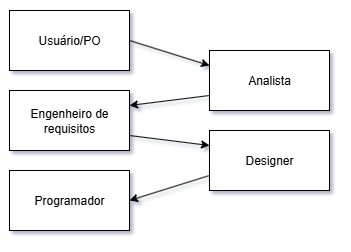
\includegraphics[width=0.8\textwidth]{Images/draw/fluxo_info.png}
  \caption{cadeia de tradução de requisitos segundo Constantine \(1979\).}
  \label{fig:cadeia_traducao}
\end{figure}

Cada etapa dessa cadeia implica na perda ou distorção de parte do significado original do usuário, o que pode resultar em comportamentos apenas próximos ao desejado. Diante disso, os autores propõem o projeto estruturado, cujo ponto inicial é a clareza e a visibilidade das decisões e atividades envolvidas, promovendo uma compreensão compartilhada e garantindo que o design reflita as intenções originais do sistema.

\subsection{Problematização}

Com o mesmo intuito de tornar o comportamento do sistema visível e compreensível, surge a modelagem de casos de uso como um instrumento de unificação entre requisitos, design e usabilidade. Segundo \textcite{booch1999unified}, nenhum sistema existe isoladamente: todo sistema relevante interage com atores, humanos ou automáticos, que esperam comportamentos previsíveis. O diagrama de casos de uso permite que analistas e desenvolvedores discutam o comportamento do sistema sem se prender aos detalhes da implementação, oferecendo uma linguagem comum e verificável para representar comportamentos.

Autores posteriores ampliaram essa discussão ao nível do código, enfatizando a necessidade de que o código não seja apenas executável, mas também compreensível. Como sintetiza \textcite{fowler2018refactoring}, “qualquer tolo escreve um código que um computador possa entender; bons programadores escrevem código que seres humanos possam entender”.

Entretanto, a legibilidade do código, por si só, não substitui a documentação de requisitos. Enquanto o código explica como o sistema se comporta, a documentação torna explícito o por que ele deve se comportar assim. Segundo \textcite{sommerville1997requirements}, a documentação de requisitos atua como um contrato conceitual entre usuários, analistas e desenvolvedores, garantindo o alinhamento entre o comportamento implementado e as expectativas de negócio. Quando essa documentação falta ou envelhece, a legibilidade do código torna-se o principal ponto de apoio para reconstruir as intenções originais, um desafio na manutenção e evolução de sistemas legados.

\subsection{Questão e hipótese}

Se o código é um texto escrito para ser lido por humanos, então suas palavras, nomes e estruturas carregam pistas úteis sobre o que o sistema faz e para quem. Partindo dessa premissa, questiona-se: é possível reconstruir casos de uso a partir do código-fonte, combinando análise estrutural e interpretação semântica automatizada?

A hipótese deste trabalho é que técnicas de representação semântica, como embeddings e Large Language Models (LLMs), quando aplicadas sobre estruturas abstratas do código, como a Abstract Syntax Tree (AST), podem permitir a reconstrução de artefatos de alto nível, como diagramas de casos de uso, mesmo na ausência de documentação formal.

\subsection{Objetivos}

O objetivo geral deste trabalho é propor um processo de redocumentação automatizada capaz de gerar diagramas de casos de uso a partir do código-fonte, preservando a semântica do sistema original.
Para isso, o método combina:

\textcite{Bruneliere2010MoDisco} o MoDisco, um framework genérico para engenharia reversa orientada por modelos (Model-Driven Reverse Engineering — MDRE). Ele sugere resumirmos os sistemas em modelos, uma estrutura mais homogênea. A principal ideia é recuperar modelos existentes no sistema. O processo é dividido em duas fases, descoberta do modelo e compreensão do modelo. Na fase de descoberta, um componente chamado discoverer extrai informações do código-fonte, dados brutos, documentações e artefatos disponíveis. Passando estas representações para uma representação uniforme da estrutura do sistema. Já na fase de compreensão, o conteúdo desse modelo é analisado e transformado em representações de alto nível, diagramas, métricas ou relatórios, que podem servir à redocumentação, à modernização de sistemas ou à análise de qualidade.

A partir dessa arquitetura, adotaremos a mesma lógica de abstração proposta por \textcite{tonella2007reverse}, utilizando uma representação sintática reduzida do código-fonte que preserva apenas os elementos essenciais ao fluxo de objetos, criações, atribuições e chamadas, e ignora instruções de controle. Essa simplificação torna possível construir a Abstract Syntax Tree (AST) como modelo intermediário, permitindo representar a estrutura sintática e os diagramas de casos de uso, permitindo representar classes, métodos, atributos e interações de forma compreensível e consistente.

Esse tipo de investigação é definido por \textcite{chikofsky1990reverse} como \textit{Redocumentation} em \textit{Reverse engineering}, ou seja, engenharia reversa com foco em redocumentação, no sentido de criar representações de abstração do sistema existente, destinadas à leitura humana, sem alterar o comportamento do software. Aqui propôe-se criar diagramas de casos de uso, preservando a semântica do sistema original, afim de compreender o comportamento observável do ponto de vista do usuário.

Além da linguagem abstrata, este trabalho incorpora informações semânticas extraídas diretamente das \textit{docstrings}, comentários e nomenclaturas do código. Esses elementos textuais são tratados como extensões dos objetos, pois também comunicam intenções, objetivos e relações entre entidades. Com o apoio de \textit{Large Language Models} (LLMs), essas evidências são analisadas de forma contextual, permitindo inferir papéis, objetivos e interações que não estão explicitamente representados nas chamadas ou estruturas do código.

Dessa forma, o processo de redocumentação combina a análise estrutural, que descreve como os objetos estão correlacionados, e a análise semântica, que interpreta o vocabulário interno do sistema revelando as intenções dos desenvolvedores. 

\subsection{Relevância}

A proposta contribui para reduzir o custo e o esforço de redocumentação de sistemas legados, um problema recorrente em ambientes corporativos e de pesquisa, nos quais o código frequentemente sobrevive à sua documentação. Ao unir análise sintática e interpretação semântica assistida por IA, o trabalho visa aproximar o entendimento do sistema à linguagem natural, recuperando a lógica de usabilidade e o comportamento observável do ponto de vista do usuário.

Além disso, o estudo resgata a importância dos casos de uso como ferramenta central na modelagem e comunicação entre equipes de desenvolvimento. Segundo \textcite{larman2002applying}, os casos de uso não apenas documentam funcionalidades, mas representam um instrumento essencial de convergência entre analistas, projetistas e programadores — especialmente em metodologias ágeis, nas quais a documentação deve ser leve, iterativa e centrada no valor entregue ao usuário. Nesses contextos, casos de uso bem definidos auxiliam na priorização de requisitos, na validação de comportamentos e na manutenção de uma visão compartilhada do sistema, mesmo em ambientes de mudança constante.

Embora a maioria dos estudos sobre Model-Driven Reverse Engineering (MDRE) e redocumentação esteja concentrada em linguagens como Java, este trabalho propõe uma abordagem direcionada à linguagem Python.

\section{AST}
Para a escolha do modo que faremos o modelo de \textit{discovery}, como mencionado no artigo \textcite{Bruneliere2010MoDisco}, analizamos 3 principais artigos: \textcite{feng2020codebert, feng2020codebert, ngo2023exploring}.

\section{Revisão literária}
Esta revisão literária foca em redocumentação através da engenharia reversa, com ênfase em recuperação de artefatos de alto nível, como diagramas UML e casos de uso a partir da análise estática. O objetivo é identificar as principais linhas de pesquisa, técnicas e limitações que fundamentam a proposta deste trabalho.

Foram analisadas publicações disponíveis nas bibliotecas digitais IEEE Xplore e ACM Digital Library, no período de 2015 a 2025, utilizando combinações de termos relacionados a reverse engineering, design recovery, use case, UML, AST, static analysis e natural language processing. Os critérios de inclusão foram artigos que propõem métodos para extrair artefatos de alto nível a partir do código-fonte e estudos que aplicam técnicas de NLP ou LLMs na recuperação de requisitos ou documentação. Foram excluídos revisões secundárias, tutoriais e trabalhos voltados exclusivamente a hardware.

\section{A Model Driven Reverse Engineering Framework for Generating High Level UML Models From Java Source Code}

Sistemas legados permanecem essenciais para a execução de operações críticas em diversas organizações, porém sua modernização representa um desafio significativo, especialmente diante da ausência de documentação arquitetural e de projeto. A \textit{Engenharia Reversa} (RE) exerce papel central nesse processo, permitindo compreender e redocumentar sistemas existentes. No entanto, as abordagens tradicionais de RE são trabalhosas, propensas a erros e, geralmente, limitadas à análise estrutural do software \textcite{Sabir2019MDRE}.

Com o surgimento da \textit{Model Driven Engineering} (MDE), surgiu uma vertente complementar: a \textit{Model Driven Reverse Engineering} (MDRE). Essa abordagem propõe representar sistemas legados em níveis mais altos de abstração por meio de modelos, reduzindo a complexidade estrutural e promovendo a reutilização, portabilidade e automação. Em geral, o processo de MDRE compreende duas etapas: (1) a extração de um modelo abstrato a partir dos artefatos-fonte e (2) a transformação desse modelo em representações de nível superior, como diagramas UML \textcite{Sabir2019MDRE}.

Diversos trabalhos anteriores contribuíram para o avanço dessa área. O \textit{MoDisco}, proposto por \textcite{Bruneliere2010MoDisco}, é um \textit{framework} extensível para engenharia reversa em Eclipse, baseado no metamodelo \textit{Knowledge Discovery Metamodel} (KDM). Apesar de sua relevância, a ferramenta limita-se à extração de aspectos estruturais, sem contemplar o comportamento dos sistemas. Outro trabalho relevante é o de Canovas2014Gra2MoL, que propõe a linguagem \textit{Gra2MoL} para transformação texto-para-modelo (\textit{Text-to-Model}, T2M), embora sem avaliação prática abrangente.  

A revisão evidencia lacunas importantes: (1) suporte limitado para extração e modelagem conjunta dos aspectos estruturais e comportamentais de sistemas legados; (2) ausência de \textit{frameworks} completos que integrem ambos os tipos de modelos; e (3) escassez de avaliações experimentais robustas \textcite{Sabir2019MDRE}.

Para superar essas limitações, \textcite{Sabir2019MDRE} propõem o \textit{Source to Model Framework} (Src2MoF), um \textit{framework} de MDRE que gera diagramas UML estruturais (classes) e comportamentais (atividades) a partir de código-fonte Java. O Src2MoF é composto por dois módulos principais: o \textit{Intermediate Model Discoverer} (IMD), responsável por criar um modelo intermediário em formato XML com base em uma árvore de sintaxe abstrata (AST); e o \textit{UML Model Generator}, que transforma esse modelo intermediário em diagramas UML por meio de regras de mapeamento do tipo \textit{Text-to-Model}.

A validação do Src2MoF foi realizada com cinco estudos de caso, incluindo o sistema de \textit{ATM} de Deitel2010Java e o caso industrial \textit{Amadeus Hospitality}. Os resultados indicam que o \textit{framework} é capaz de recuperar e modelar, de forma automatizada, tanto a estrutura quanto o comportamento de sistemas Java, superando ferramentas anteriores como o \textit{MoDisco} e o \textit{fREX}.

Os autores reconhecem, contudo, algumas limitações: o suporte atual é restrito à linguagem Java, e certos elementos dos diagramas de atividade UML (como \textit{merge nodes} e \textit{fork nodes}) ainda não são tratados. Como trabalhos futuros, pretendem estender o Src2MoF para outras linguagens, como C\#, e incorporar novos tipos de diagramas UML (sequência e componentes), ampliando a aplicabilidade do \textit{framework} em contextos de modernização de sistemas legados.

\section{Escolha dos repositórios}
Para análise foram escolhidos três repositórios independentes, dois de David Beazley e um de Brandon Rhodes, duas referências em linguagem Python. Os repositórios de David Beazley possui uma documentação completa no próprio repositório, facilitando a compreensão do software construido. Já o repositório do Brandon Rhodes não contém documentação, contudo o conteúdo é a portabilidade do jogo Colossal Cave Adventure de Fortran para Python.

\subsection{Colossal Cave Adventure}
Este trabalho utiliza como base uma reimplementação de \textcite{rhodes_adventure_py} em Python 3, que preserva o jogo original de Crowther e Don Woods, utilizando o arquivo de dados \texttt{advent.dat} \textcite{adventure_original_sources}. O pacote permite jogar em dois modos, no \emph{prompt} do Python e em terminal do sistema operacional. Além disso, disponibiliza \textit{walkthroughs} automatizados na pasta de testes.

\subsection{Descrição do jogo}

\textit{Colossal Cave Adventure}, também conhecido como \textit{ADVENT} ou simplesmente \textit{Adventure}, é amplamente reconhecido como o primeiro jogo de aventura baseado em texto da história, criado por Will Crowther em meados de 1975 e expandido por Don Woods em 1976. 

Ambientado em uma caverna repleta de tesouros, criaturas e labiríntos, o jogador interage por comandos de texto, como \textit{"GO NORTH"} ou \textit{"GET LAMP"}. O sistema responde com descrições que narram as consequências das ações.

Como observa \textcite{dibbell1998mytinylife}, o jogo automatiza o papel do mestre (\textit{Dungeon Master}) característico de campanhas de \textit{Dungeons and Dragons}. Suas descrições textuais simulam a fala do mestre (“\textit{YOU ARE IN A MAZE OF TWISTY LITTLE PASSAGES, ALL ALIKE}”).  

“Como qualquer programa significativo, \textit{Adventure} expressava a personalidade e o ambiente de seus autores.” \textcite{levy2010hackers}

Will Crowther e sua ex-esposa, Patricia Crowther, ambos programadores e espeleólogos, participaram do mapeamento do sistema de cavernas \textit{Mammoth Cave}. No verão de 1974, enquanto jogava campanhas de \textit{Dungeons and Dragons}, Will começou o desenvolvimento do seu jogo utilizando o Fortran. O mapa utilizado no jogo foi inspirado diretamente nos levantamentos realizados pelo casal durante as expedições à Mammoth Cave, construindo no código a estrutura real da caverna.

Como o próprio Will Crowther relata, a ideia do jogo surgiu da combinação entre suas experiências em espeleologia e seu interesse por \textit{Dungeons and Dragons}: “Eu estava envolvido em um jogo de interpretação de papéis... e tive uma ideia que combinasse o meu interesse por exploração de cavernas com algo que também fosse um jogo para as crianças...” \textcite{peterson1983genesis}.

\textcite{levy2010hackers} conta como inicia a colaboração de Donald Woods, um pesquisador da \textit{Stanford Artificial Intelligence Laboratory} (SAIL), em 1976. Após ter contato com uma prévia do jogo, Woods entrou em contato com Crowther, obteve sua permissão e passou a expandir o código. Sua versão incorporou novos puzzles, criaturas e elementos de fantasia inspirados na obra de Tolkien, além de um sistema de pontuação que estabelecia um objetivo ao jogador. A versão combinada de Crowther e Woods é um marco na história da interação humano-computador.

\subsection{}
Como o jogo não possui documentação original, utilizei o artigo de \textcite{jerz2007colossal} como referência para compreender a estrutura e o funcionamento do código. O autor recupera e examina o código-fonte escrito por Will Crowther, a partir de um backup preservado no SAIL. Jerz descreve as seis tabelas centrais que organizam os dados do jogo: descrições longas, rótulos curtos das salas, dados de mapa, vocabulário agrupado, estados estáticos e eventos ou dicas.  

Essa arquitetura de dados é mantida na reimplementação em Python, embora expandida para doze seções, resultado da integração da versão de Don Woods \textcite{rhodes_adventure_py}. A leitura e o processamento dessas tabelas ocorrem por meio do arquivo \texttt{advent.dat}, que preserva a semântica e a estrutura do código original. 

As seis tabelas descritas por Crowther estruturam o mundo do jogo e suas interações:
\begin{enumerate}
    \item \textbf{Long Descriptions}: textos descritivos longos que definem os ambientes e estados narrativos;
    \item \textbf{Short Room Labels}: nomes curtos usados internamente para identificar locais e facilitar a navegação;
    \item \textbf{Map Data}: conexões topológicas entre os ambientes e as direções de movimento possíveis;
    \item \textbf{Grouped Vocabulary Keywords}: agrupamento de palavras-chave e comandos interpretados pelo sistema;
    \item \textbf{Static Game States}: variáveis e condições fixas que controlam a lógica do jogo;
    \item \textbf{Hints and Events}: mensagens de ajuda, eventos dinâmicos e respostas a situações específicas.
\end{enumerate}

As outras seis adicionadas na versão em colaboração com Woods são:

\begin{enumerate}
  \item \emph{Object locations} — localização dos objetos;
  \item \emph{Action defaults} — mensagens padrão ligadas a verbos de ação;
  \item \emph{Liquid assets / flags} — \texttt{COND} por sala (luz, líquidos, restrições do pirata, bits de dicas);
  \item \emph{Class messages} — faixas de pontuação e mensagens de classificação do jogador;
  \item \emph{Hints} — dicas (turnos necessários, penalidade, pergunta e resposta);
  \item \emph{Magic messages} — mensagens de inicialização e manutenção.
\end{enumerate}

\paragraph{Tabela 1 – Long Descriptions.}  
A Tabela 1 contém descrições extensas dos ambientes do jogo. Com entradas identificadas de 1 a 140, ela define os textos apresentados ao jogador em diferentes locais. Cada linha representa uma sala ou estado narrativo. Parte dessas descrições refere-se diretamente a locais da caverna, como o trecho “\textit{YOU ARE STANDING AT THE END OF A ROAD BEFORE A SMALL BRICK BUILDING}”, enquanto outras descrevem situações de falha ou eventos inesperados, como “\textit{YOU ARE AT THE BOTTOM OF THE PIT WITH A BROKEN NECK}”.  

Exemplos:  
\begin{itemize}
    \item 1	\textit{AROUND YOU IS A FOREST.  A SMALL STREAM FLOWS OUT OF THE BUILDING AND DOWN A GULLY}.
    \item 2	\textit{YOU HAVE WALKED UP A HILL, STILL IN THE FOREST.  THE ROAD SLOPES BACK DOWN THE OTHER SIDE OF THE HILL.  THERE IS A BUILDING IN THE DISTANCE.}
    \item 3	\textit{YOU ARE INSIDE A BUILDING, A WELL HOUSE FOR A LARGE SPRING.}
\end{itemize}

\paragraph{Tabela 2 – Short Room Labels.}  
A Tabela 2 contém rótulos curtos correspondentes às localizações/ambientes do jogo. Com entradas numeradas de 1 a 130, nem todas as salas ou estados definidos em \textit{Long Descriptions} possuem equivalentes resumidos.  

Exemplos:  
\begin{itemize}
    \item 1 \textit{YOU'RE AT END OF ROAD AGAIN.}
    \item 3 \textit{YOU'RE INSIDE BUILDING.}
    \item 18 \textit{YOU'RE IN NUGGET OF GOLD ROOM.}
    \item 19 \textit{YOU'RE IN HALL OF MT KING.}
\end{itemize}

\paragraph{Tabela 3 – Map Data.}
A Tabela 3 codifica a topologia do mundo do jogo e as regras de navegação, funcionando como um grafo dirigido rotulado. A primeira coluna indica o ambiente em que o jogador se encontra, a segunda define o ambiente de destino, e as colunas subsequentes agrupam os vocabulários que podem ser utilizados para realizar a transição entre os dois pontos. O mapeamento dos vocabulários é definido na Tabela 4.  

Em alguns casos, o valor do destino representa uma condição especial, e não uma simples sala. Se o número de destino for maior que 500, o jogo exibe uma mensagem da Tabela 6 e o jogador permanece no mesmo local; Se estiver entre 300 e 500, o valor indica um salto especial para um trecho de código do jogo.
   
Exemplos:
\begin{itemize}
  \item 1  2  2  44  29: o jogador se desloca do ambiente 1 ao aombiente 2, se utilizados os comando 2, 44 ou 29. 
  \item 3  1  3  11  32  44: o jogador se desloca do ambiente 2 ao ambiente 1 se utilizados os comando 3, 11, 32 ou 44.
\end{itemize}

\paragraph{Tabela 4 – Grouped Vocabulary Keywords.}
No código original em Fortran, toda entrada de texto era truncada nos cinco primeiros caracteres, de modo que o comando \textit{“inventory”}, por exemplo, poderia ser digitado simplesmente como \textit{“inven”}. A reimplementação em Python de \textcite{rhodes_adventure_py} preserva essa lógica.  

Os dados da tabela 4 são divididos em 4 grupos: o primeiro com id's entre 1 e 100 para movimento no jogo; com ids entre 1000 e 2000, trata de objetos manipuláveis ou características de cenário; com ids entra 2000 e 3000 são verbos de ação, se entre 3000 e 4000 são para casos especiais.

\begin{itemize}
  \item 1–100: verbos de movimento, utilizados para navegação no espaço do jogo;  
  \item 1000–2000: objetos e elementos de cenário manipuláveis;  
  \item 2000–3000: verbos de ação (\textit{carry}, \textit{attack}, \textit{drop}, etc.);  
  \item 3000–4000: verbos de casos especiais, geralmente associados a eventos ou mensagens específicas definidas na Tabela 6.  
\end{itemize}

Além dos comandos clássicos de navegação por bússola, "\textit{EAST}"/"\textit{E}", "\textit{WEST}"/"\textit{W}", "\textit{NORTH}"/"\textit{N}", "\textit{SOUTH}"/"\textit{S}", parte dos veros de movimentos são nomes de locais da caverna como "\textit{BEDQU}" (truncamento de \textit{Bedquilt}), "\textit{HOUSE}", "\textit{GATE}" e "\textit{FORES}" (\textit{forest}).

Exemplos:  
\begin{itemize}
    \item 2 \textit{ROAD}
    \item 3 \textit{ENTER}
    \item 3 \textit{DOOR}
    \item 3 \textit{GATE}
    \item 4 \textit{UPSTR}
    \item 5 \textit{DOWNS}
    \item 6 \textit{FORES}
\end{itemize}

Palavras de mesmo sentido/sinônimos possuem mesmo id, como "\textit{ENTER}", "\textit{DOOR}" e "\textit{GATE}".

\paragraph{Tabela 5 – Static Game States.}  
A Tabela 5 armazena descrições curtas que representam estados do jogo, correspondendo às mudanças permanentes no ambiente. Cada linha contém um número e uma mensagem descritiva.  

Quando o identificador está entre 1 e 100, a linha define a mensagem de inventário associada a um objeto, exemplo: “\textit{SET OF KEYS}” se refere a "\textit{KEYS}". Quando o identificador é um múltiplo de 100, a mensagem descreve uma propriedado do objeto. 

Exemplos:  
\begin{itemize}
    \item 1	SET OF KEYS
    \item 000	THERE ARE SOME KEYS ON THE GROUND HERE.
    \item 2	BRASS LANTERN
    \item 000	THERE IS A SHINY BRASS LAMP NEARBY.
    \item 100	THERE IS A LAMP SHINING NEARBY.
    \item 3	*GRATE
    \item 000	THE GRATE IS LOCKED.
    \item 100	THE GRATE IS OPEN.
\end{itemize}

\paragraph{Tabela 6 – Hints and Events.}
A Tabela 6 reúne mensagens arbitrárias usadas como dicas e como descrições de eventos pontuais. Essas mensagens não estão relacionadas a um ambiente ou objeto específicos, elas são acionadas por outras estruturas do jogo, como as tabelas 3, 4, 8 e 11.

Exemplos:
\begin{enumerate}
    \item 3	AXE AT YOU WHICH MISSED, CURSED, AND RAN AWAY.
    \item 6	NONE OF THEM HIT YOU!
    \item 13 I DON'T UNDERSTAND THAT!
    \item 24 YOU ARE ALREADY CARRYING IT!
    \item 33 I DON'T KNOW HOW TO LOCK OR UNLOCK SUCH A THING.
\end{enumerate}

\paragraph{Tabela 7 – Object Locations.}
A Tabela 7 define onde cada objeto surge no mundo do jogo e se ele é móvel ou fixo. Cada linha possui o identificador do objeto, a sala inicial, e um campo opcional que indica imobilidade (-1) ou uma segunda sala quando o objeto existe simultaneamente em dois lugares 

\begin{itemize}
  \item Sala inicial = 0: o objeto não aparece no mundo no início e só será criado por algum evento ou ação do jogador.
  \item Terceiro campo = -1: o objeto está fixo naquela sala (não pode ser carregado).
  \item Terceiro campo = número de sala: o objeto está presente em duas salas ao mesmo tempo, objetos com duas localizações são tratados como imóveis.
\end{itemize}

Exemplos:
\begin{itemize}
  \item 1 3: objeto 1 (1001 - KEY, KEYS) começam na sala 3 (INSIDE BUILDING).
  \item 2 3: objeto 2 (1002 - LAMP, HEADL, LANTE) começam na sala 3 (INSIDE BUILDING).
  \item 3 8 9: objeto 3 (1003 - grate) existe nas salas 8 e 9 simultaneamente (8 - YOU'RE OUTSIDE GRATE, 9 - YOU'RE BELOW THE GRATE.).
  \item (9 - DOOR) (94 - YOU ARE AT ONE END OF AN IMMENSE NORTH/SOUTH PASSAGE.)
  \item 9 94 -1: objeto 9 (1009 - DOOR) é fixo na sala 94 (94 - YOU ARE AT ONE END OF AN IMMENSE NORTH/SOUTH PASSAGE.).
  \item 15 0: objeto 15 (1015 - OYSTE) começa fora do mundo e aparece mais tarde.
\end{itemize}

\paragraph{Tabela 8 – Action Defaults.}  
A Tabela 8 define o comportamento padrão dos verbos de ação, associando cada identificador de verbo ao índice da mensagem correspondente na Tabela 6. Cada linha contém dois valores: o primeiro é o número do verbo de ação, e o segundo é o identificador da mensagem padrão que deve ser exibida.

Exemplos:  
\begin{itemize}
  \item 1 24: o verbo de ação associado ao id 1 (2001 - CARRY, TAKE, KEEP, CATCH, STEAL, CAPTU, GET, TOTE) e a mensagem 24 da tabela 6 (YOU ARE ALREADY CARRYING IT!). 
  \item 6 33: o verbo de ação associado ao id 6 (2006 - LOCK, CLOSE) e a mensagem 33 da tabela 6 (I DON'T KNOW HOW TO LOCK OR UNLOCK SUCH A THING.).
  \item 7 38: o verbo de ação associado ao id 7 (2007 - LIGHT, ON) e a mensagem 38 da tabela 6 (YOU HAVE NO SOURCE OF LIGHT.). 
\end{itemize}

\paragraph{Tabela 9 – Liquid Assets, Etc.}
A Tabela 9 define os bits de condição associados a cada sala, controlando luz, líquidos, presença de inimigos e zonas de interesse para as rotinas de dicas. Cada linha contém um identificador de bit e uma lista de até vinte localizações nas quais esse bit é ativado. O jogo usa esses bits para determinar o comportamento dinâmico de cada ambiente.

\begin{itemize}
  \item 0: indica que o ambiente está naturalmente iluminado.
  \item 1: tipo de líquido usado em conjunto com o bit 2. Quando o bit 2 está ativo, este bit diferencia óleo (1) de água (0).
  \item 2: marca as salas que contêm água ou óleo.
  \item 3: impede que o pirata apareça ali, exceto quando persegue o jogador.
  \item 4: jogador tentando entrar na caverna.
  \item 5: tentativa de capturar o pássaro.
  \item 6: interação com a cobra.
  \item 7: perdido no labirinto.
  \item 8: refletindo no quarto escuro.
  \item 9: na área final Witt's End.
\end{itemize}

Exemplos:
\begin{itemize}
  \item 0 1 2 3 4 5 6 7 8 9 10 100 115 116 126: salas naturalmente iluminadas próximas à entrada.
  \item 2 1 3 4 7 38 95 113 24: presença de líquido (água ou óleo) nessas salas.
  \item 9 108: marca a área final do jogo, Witt’s End.
\end{itemize}

\paragraph{Tabela 10 – Class Messages.}
A Tabela 10 contém as mensagens de classificação do jogador de acordo com a pontuação total atingida ao final da partida. Cada linha associa um limite superior de pontuação a uma mensagem que descreve o título ou o nível de habilidade alcançado.  

Exemplos:
\begin{itemize}
  \item 35: YOU ARE OBVIOUSLY A RANK AMATEUR.  BETTER LUCK NEXT TIME.
  \item 100: YOUR SCORE QUALIFIES YOU AS A NOVICE CLASS ADVENTURER.
  \item 130: YOU HAVE ACHIEVED THE RATING: ‘EXPERIENCED ADVENTURER’.
  \item 200: YOU MAY NOW CONSIDER YOURSELF A ‘SEASONED ADVENTURER’.
  \item 250: YOU HAVE REACHED ‘JUNIOR MASTER’ STATUS.
  \item 300: MASTER ADVENTURER CLASSES C.
  \item 330: MASTER ADVENTURER CLASSES B.
  \item 349: MASTER ADVENTURER CLASSES A.
  \item 9999: ALL OF ADVENTUREDOM GIVES TRIBUTE TO YOU, ADVENTURER GRANDMASTER!
\end{itemize}

\paragraph{Tabela 11 – Hints.}
A Tabela 11 associa dicas contextuais a condições determinadas de jogo.  
Cada linha contém cinco valores:  

\begin{itemize}
  \item O primeiro valor vincula a dica a uma condição definidos na Tabela 9.
  \item O segundo valor define quantos turnos o jogador deve gastar no mesmo estado antes da dica ser oferecida.
  \item O terceiro valor representa a penalidade subtraída da pontuação total ao aceitar a ajuda.
  \item Os dois últimos valores apontam para mensagens da Tabela 6: a pergunta inicial e a resposta.
\end{itemize}

Exemplos:
\begin{itemize}
  \item 4 4 2 62 63 — Bit 4 (entrada da caverna): após 4 turnos no local, o jogo exibe a pergunta 62 (Do you need help getting inside?) e, se aceita, mostra a resposta 63 (Perhaps you should explore the grate.), descontando 2 pontos.
  \item 6 8 2 20 21 — Bit 6 (cobra): depois de 8 turnos, o jogador recebe uma dica para resolver o enigma da serpente.
  \item 7 75 4 176 177 — Bit 7 (labirinto): após 75 turnos perdido, é oferecida uma dica de saída, com penalidade de 4 pontos.
  \item 8 25 5 178 179 — Bit 8 (quarto escuro): a dica surge depois de 25 turnos, custando 5 pontos.
\end{itemize}

\paragraph{Tabela 12 – Magic Messages.}
A Tabela 12 contém as chamadas \textit{Magic Messages}, um conjunto de mensagens reservadas utilizadas pelos modos de inicialização, manutenção e administração do jogo.  
Embora seu formato seja idêntico ao da Tabela 6, elas são separadas para facilitar o acesso e o controle das rotinas especiais do sistema. Cada linha contém um identificador e um texto associado.agens internas do sistema.

Exemplos
\begin{itemize}
  \item 1 \textit{A LARGE CLOUD OF GREEN SMOKE APPEARS IN FRONT OF YOU… HE MAKES A SINGLE PASS OVER YOU WITH HIS HANDS, AND EVERYTHING FADES AWAY INTO A GREY NOTHINGNESS.}
  \item 2 \textit{EVEN WIZARDS HAVE TO WAIT LONGER THAN THAT!}
  \item 3 \textit{I'M TERRIBLY SORRY, BUT COLOSSAL CAVE IS CLOSED. OUR HOURS ARE:}
  \item 4 \textit{ONLY WIZARDS ARE PERMITTED WITHIN THE CAVE RIGHT NOW.}
\end{itemize}

\newpage

\printbibliography

\end{document}
